\section{Funcionalitats de la web}

\subsection{Calcular el total d'una compra.}

\subsection{Aplicar el descompte a $n$ productes}

\subsection{Generar un cupón}

\subsection{Filtrar productes per categoría}

\begin{verbatim}
    db.Products.find({category:"Nom de la categoria"})
\end{verbatim}

\begin{figure}
    \centering
    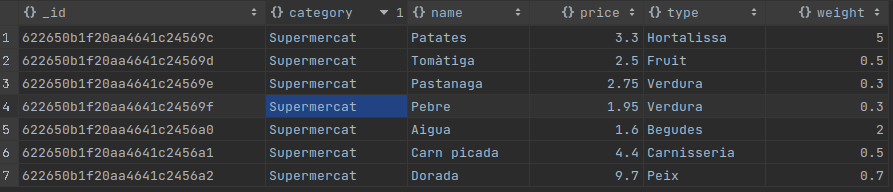
\includegraphics[width=400pt]{figures/Filtratge categories.png}
\end{figure}

\subsection{Filtrar productes per preu}

\begin{verbatim}
    db.Products.find({ price:{ $lt: 10}})
\end{verbatim}

\begin{figure}
    \centering
    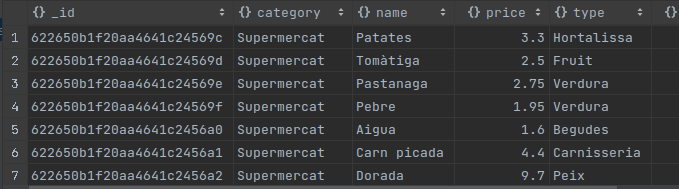
\includegraphics[width=400pt]{figures/preu.png}
\end{figure}

\subsection{Filtrar productes per tenda}

\subsection{Buscar productes}

\begin{verbatim}
    db.Products.find({name:"Nom del producte"})
\end{verbatim}

\begin{figure}
    \centering
    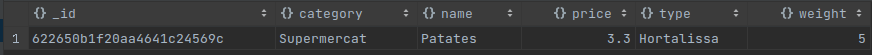
\includegraphics[width=400pt]{figures/Buscar productes.png}
\end{figure}

\subsection{Buscar productes dins una compra passada}

\begin{verbatim}
    db.Products.find({"})
\end{verbatim}

\subsection{Un usuari es canvia el nom.}

\begin{verbatim}
    db.Users.updateOne(
                        {username:"marieta12"},
                        {$set:{"username":"marieta13"}}
                      )
\end{verbatim}

\begin{figure}
    \centering
    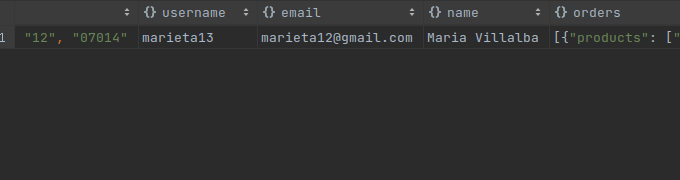
\includegraphics[width=400pt]{figures/maria.png}
\end{figure}

\subsection{}